% Configuration

\documentclass[a4paper]{article}

\linespread{1.1}

\usepackage[utf8]{inputenc} 
\usepackage[T1]{fontenc}
\usepackage[francais]{babel}
\usepackage{amsmath,amssymb}
\usepackage{amsfonts}
\usepackage{graphicx}
\usepackage{lmodern}
\usepackage{microtype}
\usepackage{hyperref}
\usepackage[margin=1.8cm]{geometry}
\usepackage{pgf,tikz}
\usepackage{mathrsfs}
\usetikzlibrary{arrows}


% Structure

\newcounter{c}
\newcounter{d}
\newcounter{r}
\newcounter{e}
\newcounter{sujet}

\newcommand{\defi}{\subparagraph{D\'efinition \arabic{c}.\arabic{d} :}\stepcounter{d}}
\newcommand{\prop}{\subparagraph{Proposition \arabic{c}.\arabic{r} :}\stepcounter{r}}
\newcommand{\thm}{\subparagraph{Th\'eor\`eme \arabic{c}.\arabic{r} :}\stepcounter{r}}
\newcommand{\demo}{\subparagraph{D\'emonstration}}
\newcommand{\cor}{\subparagraph{Corollaire \arabic{c}.\arabic{r} :}\stepcounter{r}}
\newcommand{\lem}{\subparagraph{Lemme \arabic{c}.\arabic{r} :}\stepcounter{r}}
\newcommand{\rem}{\subparagraph{Remarque :}}
\newcommand{\chapitre}[1]{\stepcounter{c}\setcounter{e}{0}\setcounter{d}{0}\setcounter{r}{0}\bigskip\noindent\textbf{\Large\arabic{sujet}.\Roman{c} - #1}\\}
\newcommand{\eq}[1]{\stepcounter{e}\begin{equation}#1\tag{\arabic{c}.\arabic{e}}\end{equation}}

% Notations

\newcommand{\Q}{\mathbb{Q}}
\newcommand{\Z}{\mathbb{Z}}
\newcommand{\N}{\mathbb{N}}
\newcommand{\R}{\mathbb{R}}
\newcommand{\C}{\mathbb{C}}
\newcommand{\E}[1]{\mathbb E\left(#1\right)}
\newcommand{\sph}{\mathbb{S}}
\newcommand{\p}{{\cal{P}}}
\newcommand{\fsp}{{\cal{F}}}
\newcommand*{\qed}{\hfill\ensuremath{\square}}
\newcommand{\x}{\mathbf x}
\newcommand{\y}{\mathbf y}
\newcommand{\e}{\mathbf e}
\newcommand{\scal}[2]{\langle#1,#2\rangle}
\newcommand{\trans}{^\text{T}\!}
\newcommand{\vertiii}[1]{{\left\vert\kern-0.25ex\left\vert\kern-0.25ex\left\vert #1 
    \right\vert\kern-0.25ex\right\vert\kern-0.25ex\right\vert}}

\newcommand{\nor}[2]{{\cal N}(#1,#2)}
\newcommand{\mat}[2]{{\cal M}_{#1\times#2}(\R)}

\newcommand{\bu}{\mathbf u}
\newcommand{\bv}{\mathbf v}
\newcommand{\bw}{\mathbf w}

\newcommand{\argmin}{\text{argmin}}

\date{}
\author{Philippe Ricka}
\title{}

\newcommand{\saut}{\vspace{0.5em}}

\begin{document}
\stepcounter{sujet}
%\maketitle

\begin{center}\huge Thermal fin\end{center}

\bigskip

\chapitre{Finite Element Approximation}


\paragraph{(a)}We consider the five PDEs :

$$-k^i\Delta\bu^i=0,i=0,...,4$$


\noindent we wish to write the variational formulation. We apply rightly the inner product by any standard test function $\bv\in X^e$ then integrate on $\Omega^i$ for each $i=0,...,4$ before taking the sum of these five terms :

$$-\sum_{i=0}^4k^i\int_{\Omega^i}\Delta\bu^i\cdot\bv=0$$


Considering $k^0=1$ and integrating by parts, we get :

$$\sum_{i=0}^4k^i\left[\int_{\Omega^i}\nabla\bu^i\cdot\nabla\bv-\int_{\Gamma^i}(\nabla\bu^i\cdot\mathbf n^i)\cdot\bv\right]=0$$


But since $\Gamma^0=\Gamma_{root}\cup\Gamma^0_{int}\cup\Gamma^0_{ext}$ and $\Gamma^i=\Gamma^i_{int}\cup\Gamma^i_{ext}$ for $i=0,...,4$, we may write :

$$\begin{array}{rl}0=&\displaystyle\sum_{i=0}^4k^i\int_{\Omega^i}\nabla\bu^i\cdot\nabla\bv-\sum_{i=1}^4k^i\left[\int_{\Gamma^i_{int}}(\nabla\bu^i\cdot\mathbf n^i)\cdot\bv+\int_{\Gamma_{ext}^i}(\nabla\bu^i\cdot\mathbf n^i)\cdot\bv\right]\\
&\\
&\displaystyle-k^0\left[\int_{\Gamma_{root}}(\nabla\bu^0\cdot\mathbf n^0)\cdot\bv+\int_{\Gamma^0_{ext}}(\nabla\bu^0\cdot\mathbf n^0)\cdot\bv\right]-k^0\int_{\Gamma^0_{int}}(\nabla\bu^0\cdot\mathbf n^0)\cdot\bv\\
&\\
=&\displaystyle\sum_{i=0}^4k^i\int_{\Omega^i}\nabla\bu^i\cdot\nabla\bv-\left[\sum_{i=1}^4k^i\int_{\Gamma^i_{int}}(\nabla\bu^i\cdot\mathbf n^i)\cdot\bv+\int_{\Gamma^0_{int}}(\nabla\bu^0\cdot\mathbf n^0)\cdot\bv\right]\\
&\\
&\displaystyle-\sum_{i=0}^4k^i\int_{\Gamma^i_{ext}}(\nabla\bu^i\cdot\mathbf n^i)\cdot\bv-\int_{\Gamma_{root}}(\nabla\bu^0\cdot\mathbf n^0)\cdot\bv
\end{array}$$


We now use the facts :
$$\begin{array}{ll}
\displaystyle\bigcup_{i=1}^4\Gamma^i_{int}=\Gamma^0_{int}&\\
\begin{array}{l}\mathbf n^i=-\mathbf n^0\\
-\nabla\bu^0\cdot\mathbf n^i=-k^i(\nabla\bu^i\cdot\mathbf n^i)\\
\end{array}&\text{ on }\Gamma^i_{int}, i=1,...,4\\
-k^i(\nabla\bu^i\cdot\mathbf n^i)=\text{Bi}~\bu^i&\text{ on }\Gamma_{ext}\\
\end{array}$$

yielding :

$$\begin{array}{rl}0=&\displaystyle\sum_{i=0}^4k^i\int_{\Omega^i}\nabla\bu^i\cdot\nabla\bv-[0]+\text{Bi}~\sum_{i=0}^4\int_{\Gamma^i_{ext}}\bu^i\cdot\bv-\int_{\Gamma_{root}}\bv
\end{array}$$

or equivalently :

$$\sum_{i=0}^4k^i\int_{\Omega^i}\nabla\bu^i\cdot\bv+\text{Bi}\int_{\partial\Omega\backslash\Gamma_{root}}\bu^i\cdot\bv=\int_{\Gamma_{root}}\bv$$

It is easy to see that it is written in the form $a(\bu,\bv;\mu)=l(\bv;\mu)$ where :

$$a(\mathbf w,\bv;\mu)=\sum_{i=0}^4k^i\int_{\Omega^i}\nabla\mathbf w^i\cdot\bv+\text{Bi}\int_{\partial\Omega\backslash\Gamma_{root}}\mathbf w^i\cdot\bv~\text{ and }~l(\bv;\mu)=\int_{\Gamma_{root}}\bv$$

are respectively a bilinear symmetric form and a linear form. We conclude by saying that $\bu^e(\mu)$ verifies : $$a(\bu^e(\mu),v;\mu)=l(v;\mu)~,~\forall\bv\in X^e$$


\paragraph{(b)}Consider :

$$J(\mathbf w)=\frac12a(\mathbf w,\mathbf w;\mu)-l(\mathbf w;\mu)$$ an let us look for its differential. It is the linear part of the following map :

$$\begin{array}{rcl}
X^e&\longrightarrow&\R\\
h&\longmapsto&J(\bw+h)
\end{array}$$

We compute :

$$\begin{array}{rl}
J(\bw+h)=&\displaystyle\frac12a(\bw+h,\bw+h;\mu)-l(\bw+h;\mu)\\
&\\
=&\displaystyle\frac12\left(a(\bw,\bw;\mu)+a(h,h;\mu)+a(\bw,h;\mu)+a(h,\bw;\mu)\right)-l(\bw;\mu)-l(h;\mu)\\
&\\
\text{since $a$ is bilinear  }~\hfill=&\displaystyle\left[\frac12(a(\bw,\bw;\mu)+a(h,h;\mu))-l(\bw;\mu)\right]+\left[a(\bw,h;\mu)-l(h;\mu)\right]\\
\end{array}$$

thus the differential of $J$ at $\bw$ is $D_\bw J(h)=a(\bw,h;\mu)-l(h;\mu)$. But according to \textbf{(a)}, for all $bv\in X^e$, we have : $a(\bu^e(\mu),\bv;\mu)=l(\bv;\mu)$, or equivalently $J(\bu^e(\mu))\equiv0$. Since $a(h,h;\mu)=\vertiii h_\mu^2\geqslant0$ for all $h\in X^e$, $\bu^e(\mu)$ is a local minimum for $J$. Since $\bu^e(\mu)$ is the only argument vanishing $D_\cdot J$, it is a global minimum for $J$.

\chapitre{Reduced-basis approximation}

\paragraph{(a)}By definition of $\bu_N\in W_N$, we have for all $\bw_N\in W_N$:

$$J(\bu_N)=\frac12a(\bu_N,\bu_N;\mu)-l(\bu_N;\mu)\leqslant\frac12a(\bw_N,\bw_N;\mu)-l(\bw_N;\mu)=J(\bw_N)$$

But :
\begin{itemize}
\item$l(\bu_N;\mu)=a(\bu(\mu),\bu_N;\mu)$
\item$l(\bw_N;\mu)=a(\bu(\mu),\bw_N;\mu)$
\end{itemize}

thus :

$$\begin{array}{rcl}
\displaystyle\frac12a(\bu_N,\bu_N;\mu)-a(\bu(\mu),\bu_N;\mu)&\leqslant&\displaystyle\frac12a(\bw_N,\bw_N;\mu)-a(\bu(\mu),\bw_N;\mu)\\
&&\\
a(\bu(\mu)-\bu_N,\bu(\mu)-\bu_N;\mu)&\leqslant&a(\bu(\mu)-\bw_N,\bu(\mu)-\bw_N;\mu)\\
&&\\
\vertiii{\bu(\mu)-\bu_N}_\mu&\leqslant&\vertiii{\bu(\mu)-\bw_N}_\mu
\end{array}$$

\paragraph{(b)}We have respectively :

$$\left\{\begin{array}{l}
T_{root N}(\mu)=l(\bu_N(\mu);\mu)\\
T_{root}(\mu)=l(\bu(\mu);\mu)
\end{array}\right.$$

thus :

$$\begin{array}{rl}
T_{root}(\mu)-T_{rootN}(\mu)=&l(\bu(\mu);\mu)-l(\bu_N(\mu);\mu)\\
=&l(\bu{\mu};\mu)-l(\bu_N(\mu);\mu)+l(\bu_N(\mu);\mu)-l(\bu_N(\mu);\mu)\\
=&a(\bu(\mu),\bu(\mu);\mu)-a(\bu(\mu),\bu_N(\mu);\mu)+a(\bu_N(\mu),\bu_N(\mu);\mu)-a(\bu_N(\mu),\bu(\mu);\mu)\\
=&a(\bu(\mu),\bu(\mu);\mu)-2a(\bu(\mu),\bu_N(\mu);\mu)+a(\bu_N(\mu),\bu_N(\mu);\mu)\\
=&a(\bu(\mu)-\bu_N(\mu),\bu(\mu)-\bu_N(\mu);\mu)\\
=&\vertiii{\bu(\mu)-\bu_N(\mu)}_\mu^2
\end{array}$$

\paragraph{(c)}We know that for all $\bw_N\in W_N$, the following holds :

$$a(\bu_N(\mu),\bw_N;\mu)=l(\bw_N;\mu)$$

Moreover, $\bu_N(\mu)=\displaystyle\sum_{i=1}^N\underline{\bu}_N^ia\xi_i$ so we can write for all $j=1,...,N$ :

$$a(\bu_N(\mu),\xi_j;\mu)=\sum_{i=1}^N\underline{\bu}_N^ia(\xi_i,\xi_j;\mu)=l(\xi_j;\mu)$$

We build the matrices $\underline A_N(\mu), \underline F_N(\mu)$ and $\underline L_N$ whose coefficients are defined by : 

$$\underline{A}_N(\mu)_{ij}=a(\xi_i,\xi_j;\mu)\text{ and }\underline{F}_N(\mu)_j=l(\xi_j;\mu)\text{ and }\underline L_N^i=\int_{\Gamma_{root}}\xi_i$$

such that : 

$$\underline A_N(\mu)\cdot\underline\bu_N(\mu)=\underline F_N(\mu)$$

$$T_{rootN}(\mu)=\int_{\Gamma_{root}}\bu_N(\mu)=\sum_{i=1}^N\underline\bu_N(\mu)\int_{\Gamma_{root}}\xi_i=\underline L_N^T\cdot\underline\bu_N$$

Packing the shapshots' components into an $\mathcal N\times N$ matrix $Z$ yields :

$$\underline A_N(\mu)=Z^T\cdot\underline A_\mathcal{N}(\mu)\cdot Z\text{ and }\underline F_N(\mu)=Z^T\cdot\underline F_\mathcal{N}(\mu)\text{ and }\underline L_N=Z^T\cdot\underline L_\mathcal N$$

\paragraph{(d)}We know that :

$$a(\bw,\bv;\mu)=\sum_{i=0}^4k^i\int_{\Omega^i}\nabla\bw\cdot\nabla\bv+\text{Bi}\int_{\partial\Omega\backslash\Gamma_{root}}\bw\bv=\sum_{i=1}^5\mu_i\int_{\Omega^{i-1}}\nabla\bw\cdot\nabla\bv+\mu_6\int_{\partial\Omega\backslash\Gamma_{root}}\bw\bv$$

Let :

$$\begin{array}{llr}
\theta^q(\mu)=\mu_q,&a^q(\bw,\bv)=\int_{\Omega^{q-1}}\nabla\bw\cdot\nabla\bv,&q=1,...,5\\
\theta^6(\mu)=\mu_6,&a^6(\bw,\bv)=\int_{\partial\Omega\backslash\Gamma_{root}}\bw\bv&
\end{array}$$

in such a way we can rewrite :

$$a(\bw,\bv;\mu)=\sum_{q=1}^6\theta^q(\mu)a^q(\bw,\bv)~,~\forall\bw,\bv\in X,~\forall\mu\in\mathcal D.$$

We now build the matrices $\underline A^{\mathcal Nq}\in\mat{\mathcal N}{\mathcal N}$ and $\underline A^q_N\in\mat NN$ whose coefficients are :

$$\underline A^{\mathcal Nq}_{ij}=a^q(\varphi_i,\varphi_j)\text{ and }\underline A^q_N=(\underline A^q_{Nij})_{ij}=(a^q(\xi_i,\xi_j))_{ij}=Z^T\cdot\underline A^\mathcal N\cdot Z=\sum_{q=1}^6\theta^q(\mu)Z^T\cdot\underline A^{\mathcal Nq}\cdot Z$$

where $\varphi_i$ denotes the $i$th FEM basis function. This yields the following two decompositions :

$$\underline A^\mathcal N(\mu)=\sum_{q=1}^6\theta^q(\mu)\underline A^{\mathcal Nq}\text{ and }\underline A_N(\mu)=\sum_{q=1}^6\theta^q(\mu)\underline A_N^q.$$

\paragraph{(e)}Let $\bar\mu\in\mathcal D$ be a fixed parameter. We endow $X^e$ with the subsequent inner product : $(\bu,\bv)_{X^e}=a(\bu,\bv;\bar\mu)$ and the associated norm $\|\cdot\|_{X^e}:\bv\in X^e\mapsto\sqrt{(\bv,\bv)_{X^e}}$. We now suppose the basis $(\xi_i)_{i=1,...,N}$ is orthonormalized with respect to this inner product. Note that it is not necessarily orthonormal with respect to another inner product $a(\cdot,\cdot;\mu),~\mu\neq\bar\mu$.

The condition number of a matrix is the quotient of its largest eigenvalue by its least one. Assume we have $\underline A_N(\mu)$'s eigenvalues $\lambda_1\geqslant...\geqslant\lambda_N$ sorted in decreasing order. Thus we have :

$$\text{cond}(\underline A_N(\mu))=\frac{\lambda_1}{\lambda_N}$$
\newpage
Since $W_N\simeq\R^N$, the least and the largest eigenvalues verify :

$$\lambda_N(\mu)=\inf_{\bv_N\in W_N}\frac{\underline\bv_N^T\cdot\underline A_N(\mu)\cdot\underline\bv_N}{\underline\bv_N^T\cdot\underline\bv_N}~\text{ and }~\lambda_1(\mu)=\sup_{\bv_N\in W_N}\frac{\underline\bv_N^T\cdot\underline A_N(\mu)\cdot\underline\bv_N}{\underline\bv_N^T\cdot\underline\bv_N}$$

On the other hand, the continuity and the coercivity constants are defined by similar quotients, namely :

$$\gamma(\mu)=\sup_{\bv,\bw\in X^e}\frac{a(\bv,\bw;\mu)}{\|\bv\|_{X^e}\|\bw\|_{X^e}}~\text{ and }~\alpha(\mu)=\inf_{\bv\in X^e}\frac{a(\bv,\bv;\mu)}{\|\bv\|^2_{X^e}}$$

Let us compute :

$$\begin{array}{rll}
\alpha(\mu)=&\displaystyle\inf_{\bv\in X^e}\frac{a(\bv,\bv;\mu)}{\|\bv\|_{X^e}}&\\
&&\\
\leqslant&\displaystyle\inf_{\bv_N\in W_N}\frac{a(\bv_N,\bv_N;\mu)}{\|\bv_N\|_{X^e}^2}&\text{ since }W_N\subset X^e\\
&&\\
=&\displaystyle\inf_{\bv_N\in W_N}\frac{\underline\bv_N^T\cdot\underline A_N(\mu)\cdot\underline\bv_N}{\sum_{i,j=1}^N\underline\bv_N^i\underline\bv_N^j(\xi^i,\xi_j)}\\
&&\\
=&\displaystyle\inf_{\bv_N\in W_N}\frac{\underline\bv_N^T\cdot\underline A_N(\mu)\cdot\underline\bv_N}{\underline\bv_N^T\cdot\underline\bv_N}&\text{ since }(\xi_i)_{i=1,...,N}\text{ is orthonormal}\\
&&\\
=&\lambda_N(mu)&\\
&&\\
\gamma(\mu)=&\displaystyle\sup_{\bv,\bw\in X^e}\frac{a(\bv,\bw;\mu)}{\|\bv\|_{X^e}\|\bw\|_{X^e}}&\\
&&\\
\geqslant&\displaystyle\sup_{\bv_N,\bw_N\in W_N}\frac{a(\bv_N,\bw_N;\mu)}{\|\bv_N\|_{X^e}\|\bw_N\|_{X^e}}&\text{ since }W_N\subset X^e\\
&&\\
=&\displaystyle\sup_{\bv_N,\bw_N\in W_N}\frac{\underline\bv_N^T\cdot\underline A_N(\mu)\cdot\underline\bw_N}{\sqrt{\sum_{i,j=1}^N\underline\bv_N^i\underline\bv_N^j(\xi^i,\xi_j)}\sqrt{\sum_{i,j=1}^N\underline\bw_N^i\underline\bw_N^j(\xi^i,\xi_j)}}\\
&&\\
\geqslant&\displaystyle\sup_{\bv_N\in W_N}\frac{\underline\bv_N^T\cdot\underline A_N(\mu)\cdot\underline\bv_N}{\sum_{i,j=1}^N\underline\bv_N^i\underline\bv_N^j(\xi^i,\xi_j)}&\\
&&\\
=&\displaystyle\sup_{\bv_N\in W_N}\frac{\underline\bv_N^T\cdot\underline A_N(\mu)\cdot\underline\bv_N}{\underline\bv_N^T\cdot\underline\bv_N}&\text{ since }(\xi_i)_{i=1,...,N}\text{ is orthonormal}\\
&&\\
=&\lambda_1(\mu)&
\end{array}$$

Since $\lambda_1(\mu)\leqslant\gamma(\mu)$ and $\alpha(\mu)\leqslant\lambda_N(\mu)$, the following result is proved : $$\text{cond}(\underline A_N(\mu))=\frac{\lambda_1(\mu)}{\lambda_N(\mu)}\leqslant\frac{\gamma(\mu)}{\alpha(\mu)}.$$



\newpage
% Sujet 2
\stepcounter{sujet}
\setcounter{c}{0}

\chapitre{Reduced basis approximation}

\paragraph{1 (a)}During the online process, we have to :
\begin{itemize}
\item build $A_N(\mu) = \displaystyle\sum_{q=1}^{Q_a}\theta_q(\mu)A_n^q\rightsquigarrow Q_a\times N^2$ products,
\item solve linear system associated with $A_N(\mu)\rightsquigarrow\mathcal N^3$ with Gauss' method,
\item compute $T_{root N}(\mu) = L_N^T\cdot \bu_N(\mu)\rightsquigarrow N$ products.
\end{itemize}

The complexity is of order $Q_aN^2+N^3+N$. It is clear that it does not depend on $\mathcal N$.

\paragraph{(b) (1)}In MatLab, our parameter array will look like {\tt(1,mu,mu,mu,mu,0.1)}.  For a sample size $N=8$, we have the following condition numbers : \begin{center}\begin{tabular}{|c|c|c|}\hline& not ortho.&ortho.\\\hline$\mu=1$&$2.7527~10^{11}$&$1$\\\hline$\mu=10$&$1.3465~10^{11}$&$9.9286$\\\hline\end{tabular}\end{center}

If we do not orthonormalize $Z$, its $i$th component is $u(\mu_i)$ so in this representation, $u(\mu_1)=(1,0,...,0)\in\R^8$. The same phenomenon happens with each value of $q$ : $u(\mu_q)=e_q$ where $e_q$ denotes the $q$th canonical basis vector of $\R^8$.


If we orthonormalize the basis of the RB space, we note the only non-zero component of $u(\mu_q)$ are the $q$ firsts. This comes from the construction of $\zeta_q$ as a linear combination of $u(\mu_l),~l=1,...,q$. The concatenation of these basis vectors will result in an upper triangular matrix.

\paragraph{(2)} For $N=8$ and $\mu = (1,5~;~1,5~;~1,5~;~1,5~;~1~;~0,1)$, we find a $T_{root}\simeq  1,5310749539187338\simeq  1,53107$.


\paragraph{(3)} Here we plot the maximum relative error between FE and RB soutions in energy norm (blue) and between FE and RB outputs (red) for $N=1,...,8$ commited amongst the set $\Xi_{test}=0.1:0.1:100$.
\begin{center}
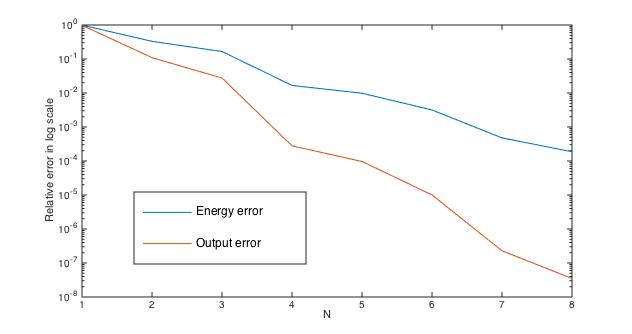
\includegraphics[width=11cm,trim={0cm 0cm 0cm 0cm},clip]{max_rel_err.jpg}
\end{center}


\paragraph{(4)} The RBM online step is 18 to 24 times faster than the FEM on the problem we are studying.

\begin{center}
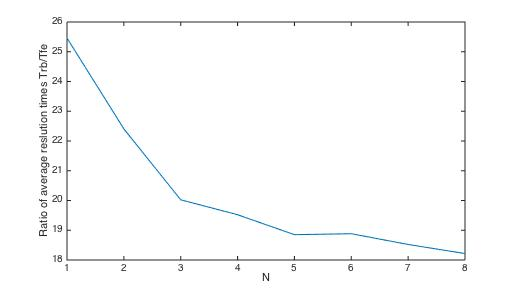
\includegraphics[width=11cm]{avg_times.jpg}
\end{center}


\paragraph{(5)} The first value of the relative output error below $0,01$ is the third one ($N=3$). This choice implies an online step running about 20 times faster in RBM.


\paragraph{(6)}  The energy and output relative errors do not seem to depend on $\mathcal N$. However, the gain in computation time is significantly affected  by $\mathcal N$. The ratio $T_{RB}/T_{FE}$ is about 50 in the medium case and about 140 in the fine case.

\paragraph{(c) (1)} In this case, we compute $T_{root}=   1,515609953667211\simeq 1,51561$.

\paragraph{(2)} We get the following maximum relative errors (as in \textbf{(b) (3)} with the same legend :

\begin{center}
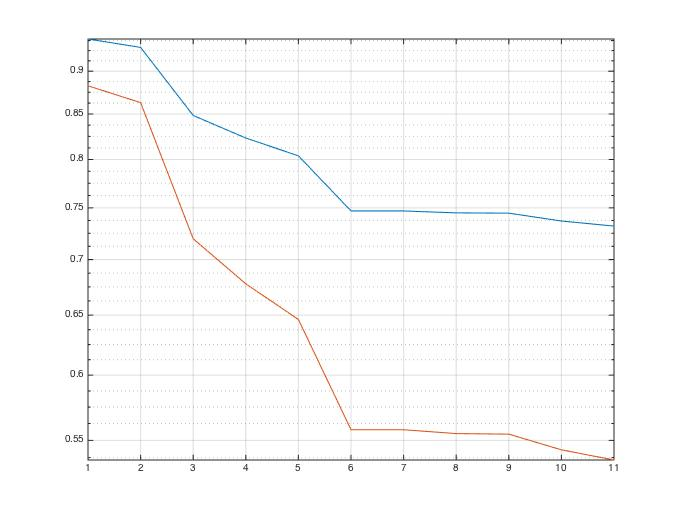
\includegraphics[width=11cm,trim={0cm 0cm 0cm 0cm},clip]{max_rel_err2.jpg}
\end{center}

\paragraph{(3)} We find a minimal cost of $   1,465520469639620$ for the fourth entry of $\Xi_{test}$, that is $Bi=0.4$.


\end{document}